\section{What is an OS?}
  \begin{frame}
    \frametitle{Operating System}
    \begin{figure}[t]
      \centering
      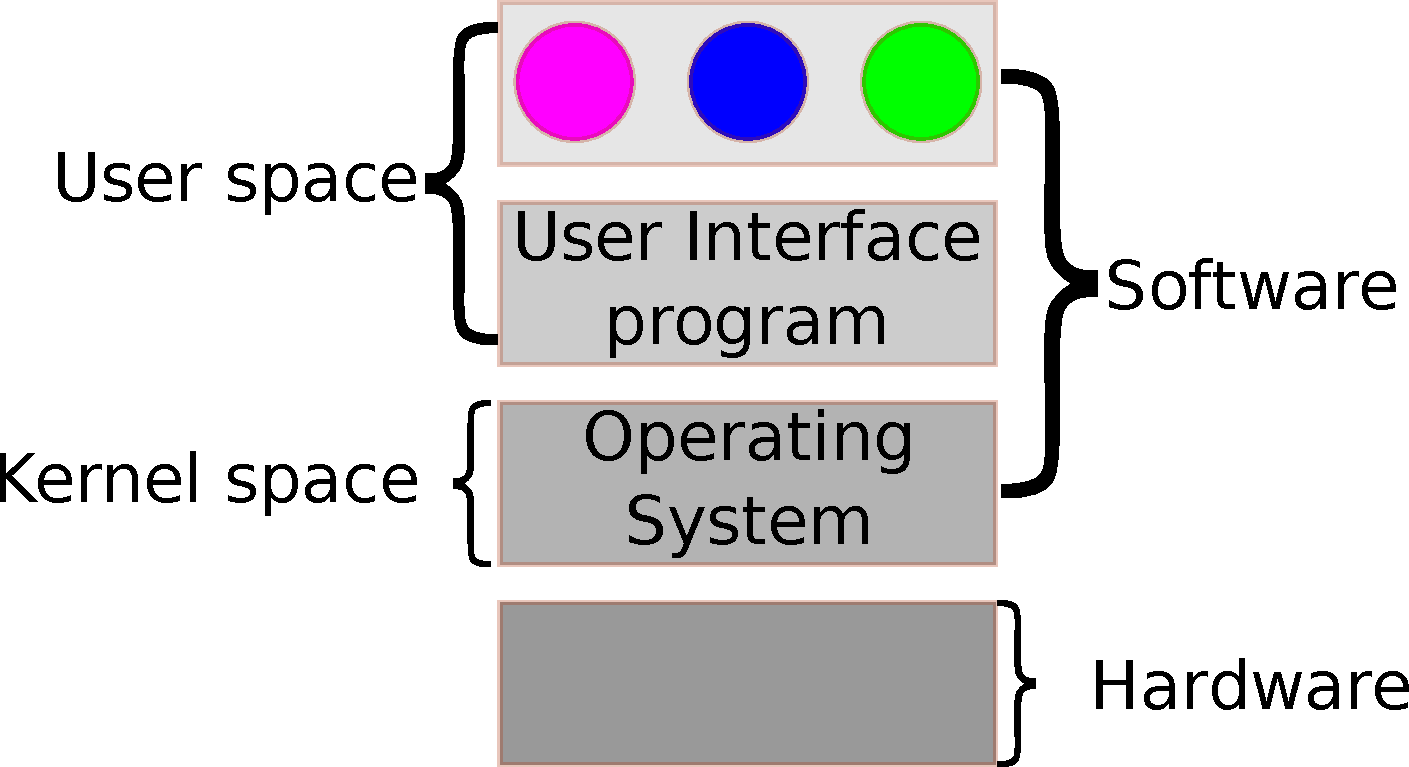
\includegraphics[height=6cm]{./imgs/os.pdf}
      \label{fig:os}
    \end{figure}
  \end{frame}

  \begin{frame}
    \frametitle{Operating System}
        \begin{block}{Two basic unrelated functions}
          \begin{itemize}
            \item provide application programmers a clean abstract set of resources,
            \item manage hardware resources.
          \end{itemize}
        \end{block}

        \begin{block}{Customers}
          OS real customers are \textbf{programs developpers}, not end users of theses developed programs.
        \end{block}
  \end{frame}

  \begin{frame}
    \frametitle{The OS as an API provider}
        \begin{block}{Abstraction challenge}
          \begin{itemize}
            \item Hardware design, as well made as it can be, only offer awkward and ugly interface to communicate.
            \item Instruction set, memory organization, I/O, bus structure are not user friendly.
            \item Programmers need not to worry about all of that thanks to the \textbf{abstraction level} provided by OS.
          \end{itemize}
        \end{block}
  \end{frame}

  \begin{frame}
    \frametitle{The OS as the resource manager}
        \begin{block}{Resource challenge}
          \begin{itemize}
            \item Orderly allocation of the processors, memory, I/O devices for all the programs competing for them.
            \item Software resources (files, DB, network access) are also managed by the OS.
            \item Multiplexing:
              \begin{itemize}
                \item Time multiplexing (CPU, printer),
                \item Space multiplexing (RAM, disk).
              \end{itemize}
          \end{itemize}
        \end{block}
  \end{frame}

  \begin{frame}
    \frametitle{The OS history}
        \begin{block}{}
          \begin{description}
            \item[1945-55] First generation: vacuum tubes
            \item[1955-65] Second generation: Transistors and Batch Systems
            \item[1965-80] Third generation: ICs\footnote{Integrated Circuit} and Multiprogramming\footnote{several programs running at once}
            \item[1980-now] Fourth generation: Personal Computers
            \item[future] Fifth generation: any suggestion?
          \end{description}
        \end{block}
  \end{frame}

  \begin{frame}
    \frametitle{The OS Zoo}
        \begin{block}{}
          \begin{description}
%\visible<1-1>{
            \item[Mainframe] Thousands of disks and millions gigabytes of data (high end web servers, servers for business-to-business transactions). Theses OS are focused on executing many jobs at once.
            \item[Server] Multiple users served at once through a network, they provide print/file/web services.
            \item[Multiprocessor] Multiples CPUs are hosted into one system (also called, according to what and how they share it: parallel computers, multicomputers, or multiprocessors).
            \item[Personal Computers] Usually used for game, spreadsheet, word processing and web browsing (laptop, desktop).
          \end{description}
        \end{block}
  \end{frame}
%}\visible<2-2>{
  \begin{frame}
    \frametitle{The OS Zoo}
        \begin{block}{}
          \begin{description}
            \item[Handheld] Small computers offering telephony, address book, web apps. They are becoming more and more sophisticated and blurring the difference between personal computers and handheld computers.
            \item[Embedded] Microwave ovens, (non-smart) TV and swatches, (not connected) cars, Bluray readers... They usual do not allow user-installed softwares.
            \item[Sensor Node] Usually small and simple to run on constraint devices with little RAM/ROM and battery life (TinyOS).
            \item[RTS\footnote{Real-Time System}] Industrial process control, avionics, military...
            \item[Smart Card] Credit card.
%}
          \end{description}
        \end{block}
  \end{frame}

  \begin{frame}
    \frametitle{Q/A}
    \begin{itemize}
      \item What is multiprogramming? %concept of performing multiple processes over a certain period of time by executing them concurrently
      %the running task keeps running until it performs an operation that requires waiting for an external event (e.g. reading from a tape) or until the computer's scheduler forcibly swaps the running task out of the CPU
      \item What is time-sharing?
      %the running task is required to relinquish the CPU, either voluntarily or by an external event such as a hardware interrupt
      \item What is real-time computing?
      %systems subject to a "real-time constraint", for example from event to system response.[1] Real-time programs must guarantee response within specified time constraints
      \item The GUI cost. Calculate the cost of the RAM (\$5/kB in 1980) for:
      \begin{itemize}
        \item 25 line per 80 row. % 2.000 bytes, about 10€ in 1980
        \item 1024 per 768 pixel with 24-bit color bitmap. % 2.359.296 bytes, about 11 k€ in 1980
      \end{itemize}
      \item What are the two main functions of an OS? % read the slides!
    \end{itemize}
  \end{frame}
